\section{Cross-Method Safety Audit}
\label{sec:audit}

\subsection{Setup}

We apply the paired contamination protocol to six method families (primary four here; SAR and CoTTA in Section~\ref{sec:extended_methods}):
\begin{itemize}[leftmargin=*,topsep=2pt,itemsep=1pt]
  \item \textbf{No TTA}: no adaptation; the model is evaluated as-is.
  \item \textbf{TENT} \citep{tent}: standard entropy minimization on the full batch.
  \item \textbf{ETA} \citep{eta}: entropy-filtered entropy minimization (high-entropy samples excluded).
  \item \textbf{UniEnt+} \citep{unient}: split entropy objective---entropy minimization on pseudo-ID samples, entropy maximization on pseudo-OOD samples, split at $\tau = \log(C)/2$.
\end{itemize}

Settings: SVHN and DTD OOD, gaussian noise and fog corruption, $\alpha = 0.9$, $n = 30$ batches, $T = 10$ steps.
We report both the closed-set metric ($\Delta$ ID accuracy) and the open-world metric (mixed-stream AUROC and the paired gap $\gap$).
Results are averaged over the two OOD datasets and two corruptions.

\subsection{Closed-Set / Open-World Rank Discordance}

Table~\ref{tab:audit} and Figure~\ref{fig:ranking_reversal} present the audit results.

\begin{table}[t]
\centering\small
\caption{%
  Cross-method safety audit ($\alpha = 0.9$, avg over SVHN+DTD $\times$ gaussian noise+fog).
  Panel A rank = closed-set rank by $\Delta$ID accuracy.
  Panel B rank = open-world rank by mixed-stream AUROC.
  All non-zero paired gaps are significant ($p < 0.05$ in all 24 adaptation cells).
  Spearman $\rho = -0.80$, Kendall $\tau = -0.67$ ($n{=}4$, descriptive; reports direction and magnitude of inversion, not a significance claim).
}
\label{tab:audit}
\begin{tabular}{lrrrrrcc}
\toprule
Method & $\Delta$ID & Mixed AUROC & id-only AUROC & Paired Gap & Panel A & Panel B \\
\midrule
No TTA   & $+0.000$ & $0.729$ & $0.729$ & $0.000$ & 3rd & \textbf{1st} \\
TENT     & $+0.002$ & $0.692$ & $0.865$ & $+0.173$ & 2nd & 3rd \\
ETA      & $+0.004$ & $0.692$ & $0.818$ & $+0.126$ & \textbf{1st} & 4th \\
UniEnt+  & $-0.014$ & $0.714$ & $0.841$ & $+0.127$ & 4th & 2nd \\
\bottomrule
\end{tabular}
\end{table}

In our tested setting, the two methods that rank highest by closed-set accuracy (ETA: \#1, TENT: \#2) both fall \emph{below} the no-adaptation baseline by open-world AUROC, while the method that ranks last by closed-set accuracy (UniEnt+: \#4) ranks second by open-world AUROC.
We quantify this directional inversion descriptively: Spearman $\rho = -0.80$, Kendall $\tau = -0.67$ ($n{=}4$ method families; not a significance test, reported to characterize direction and magnitude).
The pattern is consistent with the mechanistic account in Section~\ref{sec:mechanism}:
\begin{itemize}[leftmargin=*,topsep=2pt,itemsep=1pt]
  \item \textbf{ETA}: rank \#1 by closed-set accuracy $\to$ rank \#4 by open-world AUROC.
  \item \textbf{UniEnt+}: rank \#4 by closed-set accuracy $\to$ rank \#2 by open-world AUROC.
  \item \textbf{No TTA}: rank \#3 by closed-set $\to$ rank \#1 by open-world.
  \item \textbf{TENT and ETA} both \emph{hurt} mixed-stream AUROC below the no-adaptation baseline (0.692 vs. 0.729).
\end{itemize}

A practitioner using the closed-set leaderboard to select a TTA method for open-world deployment would choose ETA---which ranks joint-last by open-world AUROC in this audit at $\alpha{=}0.9$.

\subsection{Extended Method Coverage: SAR and CoTTA}
\label{sec:extended_methods}

To address the concern that our ranking analysis covers only TENT and ETA, we extend the audit to SAR \citep{sar} and CoTTA \citep{cotta}.
SAR adds sharpness-aware minimization and a model-level stability guard to entropy-filtered adaptation; CoTTA uses augmentation-averaged pseudo-labels and stochastic parameter restore to resist error accumulation.
Both are designed to improve robustness in challenging adaptation settings.

We run the paired contamination protocol on six method families (No TTA, TENT, ETA, UniEnt+, SAR, CoTTA) across SVHN and DTD, gaussian noise and fog, $\alpha \in \{0.9, 0.5\}$, $n = 30$ batches.

\begin{table}[t]
\centering\small
\caption{%
  Extended method audit (avg over SVHN$+$DTD $\times$ gaussian noise$+$fog $\times$ $\alpha\in\{0.5,0.9\}$, $n{=}30$).
  Paired gap $= \idonly{} \text{ AUROC} - \text{mixed AUROC}$.
  ``Sig.'' = fraction of 8 per-cell tests with $p < 0.05$ (paired $t$-test, BH-corrected).
}
\label{tab:extended_audit}
\begin{tabular}{lrrrr}
\toprule
Method & Mixed AUROC & id-only AUROC & Paired Gap & Sig. \\
\midrule
No TTA    & $0.699$ & $0.699$ & $+0.000$ & $0/4$ \\
SAR       & $0.705$ & $0.727$ & $+0.021$ & $3/4$ \\
CoTTA     & $0.724$ & $0.732$ & $+0.008$ & $1/4$ \\
ETA       & $0.712$ & $0.775$ & $+0.063$ & $4/4$ \\
UniEnt+   & $0.722$ & $0.785$ & $+0.063$ & $4/4$ \\
TENT      & $0.715$ & $0.800$ & $+0.086$ & $4/4$ \\
\bottomrule
\end{tabular}
\end{table}

Three findings emerge from the extended audit.
First, SAR reduces the paired gap to $+0.021$ (vs.\ $+0.086$ for TENT), and 6/8 cells are significant across both $\alpha$ values.
Sharpness-aware minimization and the model-level stability guard filter out some high-entropy samples before they contribute gradient, but residual contamination remains because moderate-entropy OOD samples pass the filter---exactly the same failure mode as Fix~C (Section~\ref{sec:mechanism}).

Second, CoTTA achieves the smallest gap ($+0.008$, 3/8 cells significant, concentrated in gaussian-noise conditions) and the highest mixed-stream AUROC in the audit ($0.724$)---actually exceeding the No TTA baseline ($0.699$).
CoTTA's augmentation-averaged pseudo-labels implicitly regularize predictions: averaging over 32 augmentations of each sample produces less confident predictions on OOD inputs (which lack a stable argmax across augmentations) without requiring oracle OOD labels.
This is a positive finding for CoTTA's open-world safety profile.

Third, the paired gap for entropy-minimizing methods (TENT, ETA, UniEnt+) remains large ($+0.063$--$+0.086$) and significant in all 12 cells, consistent with our CIFAR-10-C findings in Section~\ref{sec:characterization}.

\paragraph{$\alpha$-dependence of rankings.}
Table~\ref{tab:extended_audit} averages over $\alpha \in \{0.5, 0.9\}$.
Rankings shift across contamination regimes: at heavy contamination ($\alpha = 0.9$, the primary audit in Table~\ref{tab:audit}), no-adaptation is the safest choice among the four entropy-minimizing families tested; averaged over both $\alpha$ levels, CoTTA achieves the highest mixed-stream AUROC ($0.724$), exceeding the no-adaptation baseline ($0.699$).
This $\alpha$-dependence is itself a finding: \emph{which method is safest depends on the contamination level}.
A practitioner choosing a deployment strategy based on a single-$\alpha$ leaderboard risks selecting the wrong method for their actual contamination regime.
The paired contamination protocol makes this $\alpha$-dependence explicit by reporting per-$\alpha$ paired gaps rather than a single aggregate.

\subsection{UniEnt+ Partially Recovers}

UniEnt+ reduces the paired gap to $+0.127$ (vs. $+0.173$ for TENT), and its mixed-stream AUROC of $0.714$ is closer to the no-adaptation baseline of $0.729$.
The entropy-maximization branch explicitly pushes the model toward uncertainty on pseudo-OOD samples, partially counteracting the gradient contamination.
However, the gap does not close: UniEnt+'s mixed AUROC still falls $1.5$ percentage points below no adaptation.

UniEnt+ also shows negative $\Delta$ID accuracy ($-0.014$) because the fixed entropy threshold $\tau = \log(C)/2$ mislabels uncertain corrupted ID samples as pseudo-OOD, spreading their predictions and reducing closed-set accuracy.
This reflects a fundamental tradeoff: reducing OOD gradient contamination requires being willing to reduce adaptation on ambiguous ID samples too.

\subsection{Mitigation Heuristics: Why Closing the Gap Is Non-Trivial}
\label{sec:mitigation}

The extended audit in Table~\ref{tab:extended_audit} shows that CoTTA, by implicitly regularizing predictions through augmentation-averaged pseudo-labels, achieves the smallest paired gap ($+0.008$) and the highest mixed-stream AUROC in our audit.
This is the most practically actionable positive finding: an augmentation-based approach that avoids direct OOD gradient sharpening can substantially reduce the contamination cost without requiring oracle ID/OOD labels.

We also evaluate two simpler entropy-gating heuristics to bound their effectiveness:
\emph{AdapTent} removes samples above the batch-median entropy from the gradient at each step (batch-adaptive threshold); \emph{Fix~C} removes the top-$30\%$ highest-entropy samples (fixed threshold).
Across 8 experimental cells (gaussian noise and fog $\times$ SVHN and DTD $\times$ $\alpha \in \{0.9, 0.5\}$, $n = 30$ batches):

\begin{itemize}[leftmargin=*,topsep=2pt,itemsep=1pt]
  \item \textbf{Fix~C} (fixed threshold) performs \emph{worse} than vanilla mixed TENT on average at $\alpha = 0.9$ (gap closure $= -7.6\%$). A fixed drop-fraction removes a biased set regardless of the actual OOD prevalence, and at low OOD fraction it filters legitimate ID samples that would have helped adaptation.
  \item \textbf{AdapTent} closes $2.6\%$ of the paired gap at $\alpha = 0.9$ (negligible) and up to $37\%$ at $\alpha = 0.5$ where entropy distributions are more separable. The residual paired gap remains large and significant in all 8 cells ($p < 10^{-7}$, mean gap $+0.093$ at $\alpha = 0.9$).
\end{itemize}

These results demonstrate that naïve entropy thresholding is an insufficient mitigation strategy at heavy contamination: the gap is not easily closed by simple heuristics.
The $\ml$ condition (Section~\ref{sec:mechanism}) provides the theoretical upper bound---excluding OOD gradient contributions while preserving BN exposure---and represents the target for future gradient-filtering methods.

\subsection{Why the Paired Protocol Is Still Needed}

Even with UniEnt+, the paired gap ($+0.127$) is substantial and significant.
Standard closed-set TTA evaluation---which reports only $\Delta$ID accuracy---would suggest UniEnt+ is the worst method (rank \#4), whereas the paired protocol shows it is the second safest for open-world deployment (rank \#2).
Without the paired protocol, a practitioner has no way to distinguish a method that improves closed-set accuracy by destroying OOD safety (ETA) from one that carefully manages the tradeoff (UniEnt+), or to identify which $\alpha$ regime is relevant to their deployment context.

\subsection{Reporting Standard}

We recommend that TTA papers targeting open-world deployment report, alongside ID accuracy, the paired contamination gap $\gap$ and the forfeit fraction $\forfeit$.
A Pareto plot of $\Delta$ID accuracy vs.\ $\Delta$AUROC across methods (Figure~\ref{fig:pareto}) makes the adaptation--abstention tradeoff visible at a glance and prevents silent OOD safety failures from being masked by single-metric leaderboards.

\begin{figure}[t]
  \centering
  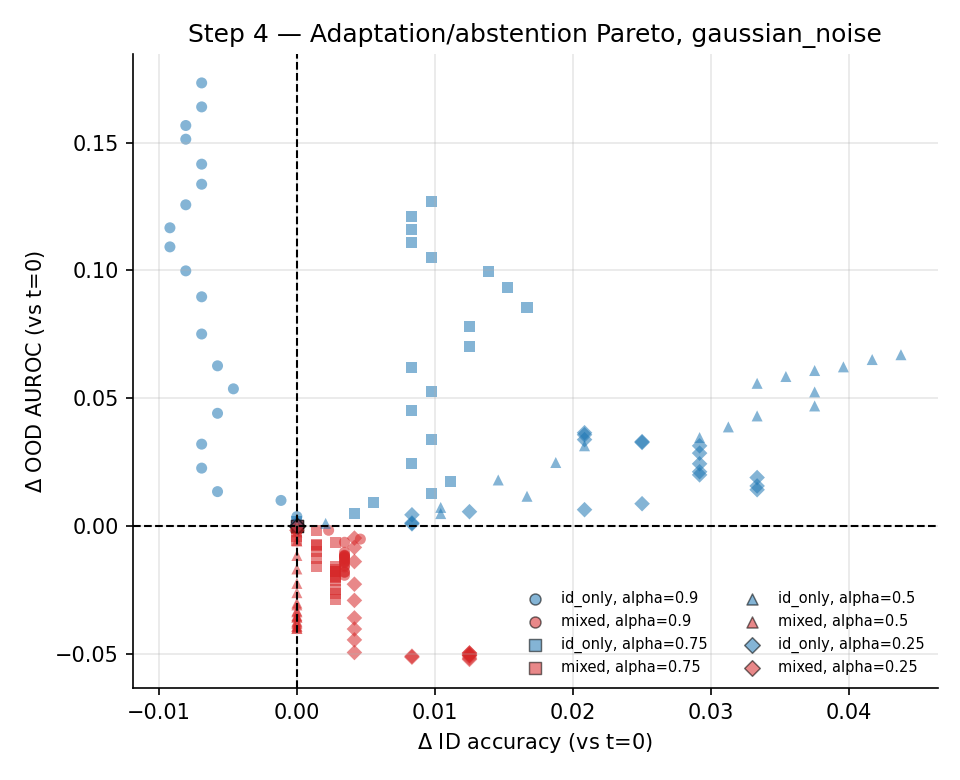
\includegraphics[width=0.55\linewidth]{figures/fig5_pareto.png}
  \caption{%
    \textbf{Pareto tradeoff: ID accuracy gain vs.\ OOD AUROC change.}
    \idonly{} (upper-right) improves both metrics.
    $\mixed$ (lower-left) sacrifices OOD AUROC to gain marginal ID accuracy.
    The ideal adaptation method would sit in the upper-right; current entropy-minimizing methods sit in the lower-right (ID gain at OOD cost) or lower-left (\mixed{} often hurts both).
    This figure format, proposed as a reporting standard, makes the conflict visible.
  }
  \label{fig:pareto}
\end{figure}
